% !TeX program = xelatex
\documentclass[12pt,a4paper]{article}
\usepackage{fontspec}
\setmainfont{Times New Roman}[Path=C:/Windows/Fonts/,UprightFont=times.ttf,BoldFont=timesbd.ttf,ItalicFont=timesi.ttf,BoldItalicFont=timesbi.ttf]
\usepackage{amsmath,amssymb,amsfonts}
\usepackage[left=1.5cm,right=1.5cm,top=1.4cm,bottom=1.6cm,headheight=17pt]{geometry}
\usepackage{enumitem,array,graphicx,tikz,fancyhdr,needspace}
\usetikzlibrary{arrows.meta,calc,patterns}
% Sửa số đề và số trang đề thực tế sau khi biên dịch/tách PDF.
\newcommand{\soDe}{6}
\newcommand{\soTrangDe}{4}
\newcommand{\maDe}{\ifnum\soDe<1000 0\fi\ifnum\soDe<100 0\fi\ifnum\soDe<10 0\fi\soDe}
\pagestyle{fancy}
\fancyhf{}
\lhead{\small\textbf{ÔN TẬP GIỮA KÌ I}}
\rhead{\small\textit{Biên soạn: Dương Gia Bảo}}
\rfoot{\small Trang \thepage/\soTrangDe\ - Mã đề: \maDe}
\renewcommand{\headrulewidth}{0.4pt}
\fancypagestyle{answers}{\rfoot{\small Trang \thepage\ - Mã đề: \maDe}}
\fancypagestyle{firstpage}{\fancyhead{}\renewcommand{\headrulewidth}{0pt}}
\setlength{\parindent}{0pt}
\setlength{\parskip}{2.5pt}
\setlength{\emergencystretch}{1em}
\setlist[enumerate,1]{label=\textbf{Câu \arabic*:},leftmargin=*,itemsep=5pt,topsep=2pt}
\setlist[enumerate,2]{label=\alph*),leftmargin=*,itemsep=2pt,topsep=2pt}
\newcommand{\bonpa}[4]{\par\nobreak\smallskip\nobreak\noindent
\begin{tabular}{@{}p{0.47\linewidth}p{0.47\linewidth}@{}}
\textbf{A.} #1 & \textbf{B.} #2\\[8pt]
\textbf{C.} #3 & \textbf{D.} #4\end{tabular}}
\newcommand{\loigiai}[1]{\par\medskip\Needspace{4\baselineskip}\noindent\textbf{#1}\par\nobreak}
\newcommand{\otraloi}{\par\nobreak\smallskip\noindent\textit{Trả lời:}\quad\fbox{\rule{0pt}{11pt}\makebox[0.3cm]{}}\,\fbox{\rule{0pt}{11pt}\makebox[0.3cm]{}}\,\fbox{\rule{0pt}{11pt}\makebox[0.3cm]{}}\,\fbox{\rule{0pt}{11pt}\makebox[0.3cm]{}}}
\begin{document}
\thispagestyle{firstpage}
\noindent
\begin{minipage}[t]{0.35\textwidth}
    \centering
    {\fontsize{13}{15}\selectfont\textbf{ÔN TẬP GIỮA KÌ I}}\\[4pt]
    \textit{Biên soạn: Dương Gia Bảo}\\[5pt]
    \setlength{\fboxrule}{0.8pt}%
    \setlength{\fboxsep}{4pt}%
    \fbox{\begin{minipage}{0.83\linewidth}
        \centering
        {\fontsize{13}{15}\selectfont\textbf{ĐỀ ÔN TẬP}\\[2pt]\textbf{CHƯƠNG I VÀ II}}\\[4pt]
        \textit{(Đề thi gồm có \ifnum\soTrangDe<10 0\fi\soTrangDe\ trang)}
    \end{minipage}}
\end{minipage}\hfill
\begin{minipage}[t]{0.63\textwidth}
    \centering
    {\fontsize{13}{15}\selectfont\textbf{ÔN TẬP KIỂM TRA GIỮA KÌ I}\\[2pt]
    \textbf{NĂM HỌC 2026 - 2027}}\\[5pt]
    {\fontsize{14}{16}\selectfont\textbf{Môn: TOÁN - Lớp 12 (ĐỀ SỐ \soDe)}}\\[4pt]
    {\fontsize{11.5}{13}\selectfont\textit{Thời gian làm bài: 90 phút, không kể thời gian giao đề}}\\[5pt]
    \setlength{\fboxrule}{0.8pt}%
    \setlength{\fboxsep}{5pt}%
    \fbox{\makebox[3cm]{\fontsize{14}{16}\selectfont\textbf{Mã đề: \maDe}}}
\end{minipage}
\par\vspace{2pt}
\hrule height 0.6pt
\vspace{3pt}
\noindent\textit{Họ và tên học sinh:}\dotfill\hspace{1cm}\textit{Lớp:}\makebox[3.5cm]{\dotfill}
\par\vspace{2pt}
\hrule height 0.6pt
\vspace{3pt}

\section*{\large PHẦN I. Câu trắc nghiệm nhiều phương án lựa chọn}
\textit{Thí sinh trả lời từ câu 1 đến câu 12. Mỗi câu chỉ chọn một phương án.}
\begin{enumerate}
\item Cho hàm số $y=x^3-3x^2+2$. Hàm số đã cho nghịch biến trên khoảng nào dưới đây?
\bonpa{$(-\infty;0)$.}{$(0;2)$.}{$(2;+\infty)$.}{$(-1;3)$.}

\item Cho hàm số $y=-x^3+3x+1$. Điểm cực tiểu của hàm số đã cho là
\bonpa{$x=-1$.}{$x=1$.}{$x=3$.}{$x=0$.}

\item Giá trị nhỏ nhất của hàm số $f(x)=x+\dfrac{4}{x}$ trên đoạn $[1;3]$ bằng
\bonpa{$5$.}{$\dfrac{13}{3}$.}{$4$.}{$2$.}

\item Đường tiệm cận đứng và đường tiệm cận ngang của đồ thị hàm số $y=\dfrac{2x+3}{x-1}$ lần lượt có phương trình là
\bonpa{$x=1$ và $y=-3$.}{$x=2$ và $y=1$.}{$x=-1$ và $y=2$.}{$x=1$ và $y=2$.}

\item Đường tiệm cận xiên của đồ thị hàm số $y=\dfrac{x^2+2x-1}{x+1}$ có phương trình là
\bonpa{$y=x+1$.}{$y=x-1$.}{$y=x+2$.}{$y=2x+1$.}

\item Đường cong trong hình vẽ bên là đồ thị của hàm số nào dưới đây?
\par\nobreak\smallskip
\begin{minipage}[c]{0.62\linewidth}
\bonpa{$y=\dfrac{x^2+x+1}{x-1}$.}{$y=\dfrac{x^2-x+1}{x-1}$.}{$y=\dfrac{x^2-2x+2}{x-1}$.}{$y=\dfrac{-x^2+x-1}{x-1}$.}
\end{minipage}\hfill
\begin{minipage}[c]{0.36\linewidth}\centering
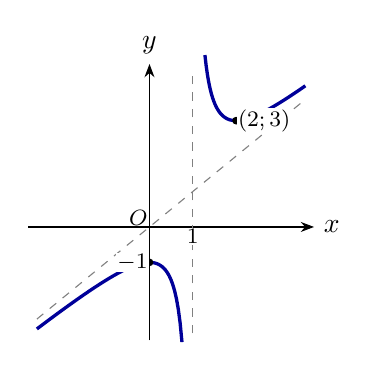
\begin{tikzpicture}[x=0.55cm,y=0.45cm,>=Stealth]
\draw[->] (-2.8,0)--(3.8,0) node[right] {$x$};
\draw[->] (0,-3.2)--(0,4.6) node[above] {$y$};
\draw[dashed,gray] (1,-3.0)--(1,4.4);
\draw[dashed,gray,domain=-2.6:3.6] plot (\x,{\x});
\draw[very thick,blue!60!black,domain=-2.6:0.75,samples=80] plot (\x,{(\x*\x-\x+1)/(\x-1)});
\draw[very thick,blue!60!black,domain=1.28:3.6,samples=80] plot (\x,{(\x*\x-\x+1)/(\x-1)});
\fill (0,-1) circle (1.4pt);\fill (2,3) circle (1.4pt);
\node[above left,fill=white,inner sep=0.5pt] at (0,0) {\footnotesize $O$};
\node[below,fill=white,inner sep=0.5pt] at (1,0) {\footnotesize $1$};
\node[left,fill=white,inner sep=0.5pt] at (0,-1) {\footnotesize $-1$};
\node[right,fill=white,inner sep=0.5pt] at (2,3) {\footnotesize $(2;3)$};
\end{tikzpicture}
\end{minipage}
\end{enumerate}

\newpage
\begin{enumerate}[start=7]
\item Một hồ nuôi cá ước tính nồng độ ôxy hòa tan trong nước (đơn vị: mg/L) sau $t$ ngày kể từ khi bắt đầu thả men vi sinh được mô hình hóa bởi hàm số $C(t)=5+\dfrac{12t}{t^2+9}$ với $t\ge 0$. Hỏi sau bao nhiêu ngày kể từ khi thả men vi sinh thì nồng độ ôxy hòa tan trong nước đạt giá trị cao nhất?
\bonpa{$2$ ngày.}{$9$ ngày.}{$3$ ngày.}{$6$ ngày.}

\item Cho hình hộp chữ nhật $ABCD.A'B'C'D'$. Tổng vectơ $\vec{BA}+\vec{BC}+\vec{BB'}$ bằng vectơ nào dưới đây?
\bonpa{$\vec{BD}$.}{$\vec{AC'}$.}{$\vec{B'D}$.}{$\vec{BD'}$.}

\item Trong không gian $Oxyz$, cho tam giác $ABC$ có $A(1;2;3)$, $B(-2;0;1)$ và $C(4;1;-1)$. Tọa độ trọng tâm $G$ của tam giác $ABC$ là
\bonpa{$(1;1;1)$.}{$(3;3;3)$.}{$(1;1;2)$.}{$(2;1;1)$.}

\item Trong không gian $Oxyz$, cho hai vectơ $\vec{a}=(2;-1;3)$ và $\vec{b}=(1;3;-2)$. Tọa độ của vectơ $\vec{u}=\vec{a}-2\vec{b}$ là
\bonpa{$(0;5;-1)$.}{$(0;-7;7)$.}{$(4;5;-1)$.}{$(0;-7;-1)$.}

\item Trong không gian $Oxyz$, cho hai vectơ $\vec{u}=(1;0;-1)$ và $\vec{v}=(0;1;1)$. Góc giữa hai vectơ $\vec{u}$ và $\vec{v}$ bằng
\bonpa{$60^\circ$.}{$45^\circ$.}{$120^\circ$.}{$135^\circ$.}

\item Trong không gian $Oxyz$, cho hai điểm $M(2;-1;4)$ và $N(4;1;3)$. Khoảng cách giữa hai điểm $M$ và $N$ bằng
\bonpa{$9$.}{$\sqrt{5}$.}{$\sqrt{17}$.}{$3$.}
\end{enumerate}

\vspace{3pt}
\section*{\large PHẦN II. Câu trắc nghiệm đúng hoặc sai}
\textit{Thí sinh trả lời từ câu 1 đến câu 4. Trong mỗi ý a), b), c), d) ở mỗi câu, thí sinh chọn đúng hoặc sai.}
\begin{enumerate}
\item Cho hàm số $y=f(x)=\dfrac{x^2-4x+5}{x-2}$.
\begin{enumerate}
\item Tập xác định của hàm số là $D=\mathbb{R}\setminus\{2\}$.
\item Đạo hàm của hàm số là $f'(x)=\dfrac{x^2-4x+3}{(x-2)^2}$.
\item Đồ thị hàm số có đường tiệm cận xiên là đường thẳng $y=x+2$.
\item Đồ thị hàm số có hai điểm cực trị $A$ và $B$. Hai điểm cực trị $A, B$ đối xứng nhau qua điểm $I(2;0)$.
\end{enumerate}
\end{enumerate}

\newpage
\begin{enumerate}[start=2]
\item Một công ty dược phẩm sản xuất một loại vắc-xin với số lượng $x$ nghìn liều trong một đợt sản xuất ($0\le x\le 120$). Tổng chi phí sản xuất (triệu đồng) được cho bởi hàm số $C(x)=x^3-90x^2+2400x+10000$. Doanh thu từ việc bán sản phẩm (triệu đồng) được cho bởi hàm số $R(x)=3600x-15x^2$. Lợi nhuận của công ty là $P(x)=R(x)-C(x)$.
\begin{enumerate}
\item Chi phí cố định ban đầu của công ty (khi chưa sản xuất sản phẩm nào) là $10000$ triệu đồng.
\item Doanh thu của công ty khi bán được $20$ nghìn liều vắc-xin là $66000$ triệu đồng.
\item Hàm số biểu thị lợi nhuận của công ty là $P(x)=-x^3+75x^2+1200x-10000$.
\item Công ty đạt lợi nhuận lớn nhất khi sản xuất $50$ nghìn liều vắc-xin.
\end{enumerate}

\item Trong không gian $Oxyz$, cho ba điểm $A(2;1;-1)$, $B(4;3;0)$ và $C(1;5;1)$.
\begin{enumerate}
\item Tọa độ của vectơ $\vec{AB}$ là $\vec{AB}=(2;2;1)$.
\item Trọng tâm $G$ của tam giác $ABC$ có tọa độ là $G(2;3;0)$.
\item Độ dài đoạn thẳng $AB$ bằng $3$.
\item Tọa độ điểm $D$ để tứ giác $ABCD$ là hình bình hành là $D(-1;3;0)$.
\end{enumerate}

\item Một khung đèn trang trí có trọng lượng $P=180\text{ N}$ được treo vào trần nhà bằng ba sợi dây cáp không dãn có độ dài bằng nhau, buộc vào trần nhà tại ba điểm $A, B, C$ và cùng hội tụ tại điểm móc $O$ của khung đèn. Chọn hệ trục tọa độ $Oxyz$ có gốc tại $O$, trục $Oz$ hướng thẳng đứng lên trên. Khi đó trọng lực tác dụng lên đèn là $\vec{P}=(0;0;-180)$ (đơn vị: N). Lực căng của ba sợi dây tác dụng lên móc treo $O$ lần lượt là $\vec{T}_1, \vec{T}_2, \vec{T}_3$. Biết rằng ba lực $\vec{T}_1, \vec{T}_2, \vec{T}_3$ đôi một vuông góc và có cùng độ lớn $|\vec{T}_1|=|\vec{T}_2|=|\vec{T}_3|=T$.
\begin{enumerate}
\item Vì khung đèn ở trạng thái cân bằng nên $\vec{T}_1+\vec{T}_2+\vec{T}_3+\vec{P}=\vec{0}$.
\item Do ba lực $\vec{T}_1, \vec{T}_2, \vec{T}_3$ đôi một vuông góc nên $|\vec{T}_1+\vec{T}_2+\vec{T}_3|^2=|\vec{T}_1|^2+|\vec{T}_2|^2+|\vec{T}_3|^2=3T^2$.
\item Độ lớn của mỗi lực căng dây là $T=60\text{ N}$.
\item Góc $\alpha$ giữa mỗi sợi dây cáp và phương thẳng đứng thỏa mãn $\cos\alpha=\dfrac{\sqrt{3}}{3}$.
\end{enumerate}
\end{enumerate}

\vspace{3pt}
\section*{\large PHẦN III. Câu trắc nghiệm trả lời ngắn}
\textit{Thí sinh trả lời từ câu 1 đến câu 6. Mỗi câu trả lời đúng thí sinh được 0,5 điểm.}
\begin{enumerate}
\item Có bao nhiêu giá trị nguyên của tham số $m$ để hàm số $y=-\dfrac{1}{3}x^3+mx^2-(2m+3)x+2027$ nghịch biến trên khoảng $(-\infty;+\infty)$?
\otraloi

\item Trong không gian $Oxyz$, cho hình hộp $ABCD.A'B'C'D'$ có $A(2;1;0)$, $B(3;4;2)$, $D(1;3;1)$ và $A'(4;1;5)$. Tìm tọa độ đỉnh $C'(x;y;z)$, sau đó tính tổng $S=x+y+z$.
\otraloi
\end{enumerate}

\newpage
\begin{enumerate}[start=3]
\item Cho hàm số $y=\dfrac{x^2+mx-1}{x+1}$. Biết rằng đồ thị hàm số có hai điểm cực trị nằm về hai phía của trục tung $Oy$. Có bao nhiêu giá trị nguyên của tham số $m\in[-6;6]$ thỏa mãn yêu cầu bài toán?
\otraloi

\item Trong không gian $Oxyz$ (với đơn vị đo trên các trục tọa độ là mét), có hai thiết bị bay không người lái (drone) $M$ và $N$ đang thực hiện chuyến bay thử nghiệm. Tại thời điểm $t$ giây ($t\ge 0$), vị trí của drone $M$ là $M(t;2;15)$ và vị trí của drone $N$ là $N(6-t;2+2t;t+9)$. Khoảng cách ngắn nhất giữa hai drone trong quá trình bay bằng bao nhiêu mét?
\otraloi

\item Một cơ sở sản xuất cần chế tạo một bồn chứa nước bằng inox dạng hình trụ kín hai đáy đặt vừa khít bên trong một tháp nước dạng hình nón có bán kính đáy $R=9\text{ cm}$ và chiều cao $H=18\text{ cm}$ (trục của bồn hình trụ trùng với trục đối xứng của tháp hình nón, mặt đáy dưới của hình trụ nằm trên mặt đáy của hình nón như hình vẽ minh họa). Bán kính đáy $r$ của bồn chứa hình trụ bằng bao nhiêu xentimét để thể tích của bồn chứa đạt giá trị lớn nhất?
\par\smallskip
\begin{center}
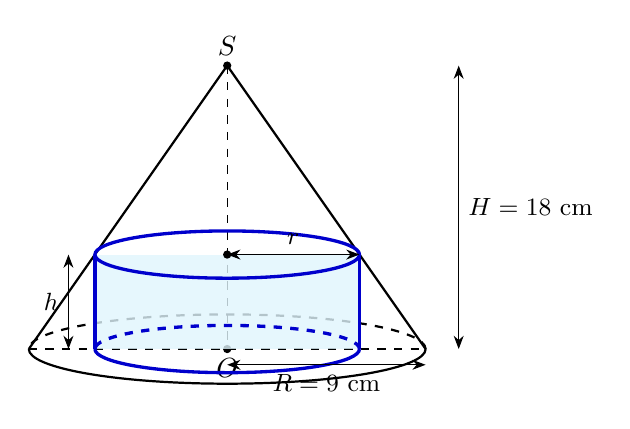
\begin{tikzpicture}[x=0.28cm,y=0.20cm,>=Stealth]
% Nón: đỉnh S(0,18), đáy bán kính 9 ở y=0
\coordinate (S) at (0,18);
\coordinate (O) at (0,0);
\draw[thick] (-9,0)--(S)--(9,0);
\draw[thick] (9,0) arc (0:-180:9 and 2.2);
\draw[dashed,thick] (9,0) arc (0:180:9 and 2.2);
\draw[dashed] (S)--(O);
\draw[dashed] (-9,0)--(9,0);
\fill (O) circle (1.5pt) node[below] {$O$};
\fill (S) circle (1.5pt) node[above] {$S$};

% Trụ: r=6, h=6 (từ y=0 đến y=6)
\fill[cyan!12,opacity=0.8] (-6,0) rectangle (6,6);
\draw[very thick,blue!80!black] (-6,0)--(-6,6) (6,0)--(6,6);
\draw[very thick,blue!80!black] (0,6) ellipse (6 and 1.5);
\draw[very thick,blue!80!black] (6,0) arc (0:-180:6 and 1.5);
\draw[dashed,very thick,blue!80!black] (6,0) arc (0:180:6 and 1.5);
\coordinate (O1) at (0,6);
\fill (O1) circle (1.5pt);

% Kích thước
\draw[<->] (0,6)--(6,6) node[midway,above] {\small $r$};
\draw[<->] (0,-1.0)--(9,-1.0) node[midway,below] {\small $R=9\text{ cm}$};
\draw[<->] (10.5,0)--(10.5,18) node[midway,right] {\small $H=18\text{ cm}$};
\draw[<->] (-7.2,0)--(-7.2,6) node[midway,left] {\small $h$};
\end{tikzpicture}
\par\vspace{2pt}{\footnotesize\textit{Hình minh họa bồn hình trụ nội tiếp tháp hình nón.}}
\end{center}
\otraloi

\item Một doanh nghiệp cần xây dựng một bể chứa nước ngầm dạng hình hộp chữ nhật không nắp có thể tích $V=60\text{ m}^3$. Đáy bể là hình chữ nhật có chiều dài gấp đôi chiều rộng. Giá thuê nhân công và vật liệu xây đáy bể là $1$ triệu đồng/$\text{m}^2$, chi phí xây bốn bức tường xung quanh là $600$ nghìn đồng/$\text{m}^2$ ($0{,}6$ triệu đồng/$\text{m}^2$). Biết chiều cao của bể không vượt quá $5\text{ m}$. Tổng chi phí thấp nhất để doanh nghiệp xây dựng bể chứa nước này bằng bao nhiêu triệu đồng?
\par\smallskip
\begin{center}
\begin{tikzpicture}[x=0.75cm,y=0.55cm,>=Stealth]
% Bể hình hộp chữ nhật đáy dài 2x, rộng x, cao h
\coordinate (A) at (0,0);
\coordinate (B) at (4.5,0);
\coordinate (C) at (6,1.2);
\coordinate (D) at (1.5,1.2);
\coordinate (Ap) at (0,2.5);
\coordinate (Bp) at (4.5,2.5);
\coordinate (Cp) at (6,3.7);
\coordinate (Dp) at (1.5,3.7);

% Mặt nước / lòng bể
\fill[cyan!15] (A)--(B)--(C)--(D)--cycle;
\fill[cyan!25,opacity=0.6] (A)--(B)--(Bp)--(Ap)--cycle;
\fill[cyan!35,opacity=0.6] (B)--(C)--(Cp)--(Bp)--cycle;

% Cạnh khuất
\draw[dashed,thick] (A)--(D)--(C);
\draw[dashed,thick] (D)--(Dp);

% Cạnh thấy
\draw[thick] (A)--(B)--(C);
\draw[thick] (Ap)--(Bp)--(Cp)--(Dp)--cycle;
\draw[thick] (A)--(Ap) (B)--(Bp) (C)--(Cp);

% Kích thước
\draw[<->] (0,-0.4)--(4.5,-0.4) node[midway,below] {\small Chiều dài: $2x$};
\draw[<->] (4.8,-0.15)--(6.3,1.05) node[midway,below right] {\small Chiều rộng: $x$};
\draw[<->] (-0.4,0)--(-0.4,2.5) node[midway,left] {\small Chiều cao: $h$};
\node at (2.7,1.3) {\small $V=60\text{ m}^3$};
\end{tikzpicture}
\par\vspace{2pt}{\footnotesize\textit{Hình minh họa bể nước ngầm hình hộp chữ nhật không nắp.}}
\end{center}
\otraloi
\end{enumerate}
\begin{center}\textbf{---------------- HẾT ----------------}\end{center}

\newpage\pagestyle{answers}
\begin{center}\Large\textbf{BẢNG ĐÁP ÁN TỔNG HỢP}\end{center}
\textbf{Phần I. Trắc nghiệm nhiều phương án lựa chọn}
\begin{center}
\renewcommand{\arraystretch}{1.5}
\begin{tabular}{|c|*{12}{c|}}\hline
Câu & 1&2&3&4&5&6&7&8&9&10&11&12\\\hline
Đáp án & B & A & C & D & A & B & C & D & A & B & C & D \\\hline
\end{tabular}
\end{center}

\textbf{Phần II. Đúng hoặc sai}
\begin{center}
\renewcommand{\arraystretch}{1.4}
\begin{tabular}{|c|c|c|c|c|}\hline
Câu & a) & b) & c) & d)\\\hline
1 & Đ & Đ & S & Đ\\\hline
2 & Đ & Đ & Đ & S\\\hline
3 & Đ & S & Đ & Đ\\\hline
4 & Đ & Đ & S & Đ\\\hline
\end{tabular}
\end{center}

\textbf{Phần III. Trả lời ngắn}
\begin{center}
\renewcommand{\arraystretch}{1.5}
\begin{tabular}{|c|c|c|c|c|c|c|}\hline
Câu & 1 & 2 & 3 & 4 & 5 & 6\\\hline
Đáp án & 5 & 18 & 5 & 6 & 6 & 54 \\\hline
\end{tabular}
\end{center}

\vspace{5pt}
\begin{center}
\textbf{THANG ĐIỂM ĐÁNH GIÁ}
\end{center}
\begin{itemize}[leftmargin=*,itemsep=2pt]
\item \textbf{Phần I:} Gồm 12 câu hỏi trắc nghiệm bốn lựa chọn. Mỗi câu trả lời đúng được \textbf{0,25 điểm}. Tổng điểm tối đa: \textbf{3,0 điểm}.
\item \textbf{Phần II:} Gồm 4 câu hỏi trắc nghiệm Đúng/Sai (mỗi câu gồm 4 ý a, b, c, d). Điểm số mỗi câu được tính như sau:
\begin{itemize}[leftmargin=2cm]
\item Thí sinh chỉ chọn chính xác $1$ ý trong $1$ câu được \textbf{0,1 điểm}.
\item Thí sinh chỉ chọn chính xác $2$ ý trong $1$ câu được \textbf{0,25 điểm}.
\item Thí sinh chỉ chọn chính xác $3$ ý trong $1$ câu được \textbf{0,5 điểm}.
\item Thí sinh chọn chính xác cả $4$ ý trong $1$ câu được \textbf{1,0 điểm}.
\end{itemize}
Tổng điểm tối đa Phần II: \textbf{4,0 điểm}.
\item \textbf{Phần III:} Gồm 6 câu hỏi trắc nghiệm trả lời ngắn. Mỗi câu trả lời đúng được \textbf{0,5 điểm}. Tổng điểm tối đa: \textbf{3,0 điểm}.
\item \textbf{Tổng toàn đề:} \textbf{10,0 điểm}. Thời gian làm bài: \textbf{90 phút}.
\end{itemize}

\newpage
\section*{\large HƯỚNG DẪN GIẢI CHI TIẾT}

\subsection*{PHẦN I. Câu trắc nghiệm nhiều phương án lựa chọn}

\loigiai{Câu 1: Chọn B.}
Hàm số $y=x^3-3x^2+2$ có đạo hàm $y'=3x^2-6x=3x(x-2)$.\\
Xét dấu đạo hàm: $y'<0 \iff 3x(x-2)<0 \iff 0<x<2$.\\
Do đó hàm số nghịch biến trên khoảng $(0;2)$.

\loigiai{Câu 2: Chọn A.}
Hàm số $y=-x^3+3x+1$ xác định trên $\mathbb{R}$.\\
Đạo hàm: $y'=-3x^2+3=-3(x^2-1)=0 \iff x=\pm 1$.\\
Đạo hàm cấp hai: $y''=-6x$.\\
- Tại $x=-1$, ta có $y''(-1)=6>0$ nên $x=-1$ là điểm cực tiểu của hàm số.\\
- Tại $x=1$, ta có $y''(1)=-6<0$ nên $x=1$ là điểm cực đại của hàm số.\\
Vậy điểm cực tiểu của hàm số đã cho là $x=-1$.

\loigiai{Câu 3: Chọn C.}
Hàm số $f(x)=x+\dfrac{4}{x}$ liên tục trên đoạn $[1;3]$.\\
Ta có $f'(x)=1-\dfrac{4}{x^2}=\dfrac{x^2-4}{x^2}$. Trên đoạn $[1;3]$, $f'(x)=0 \iff x=2$.\\
Tính các giá trị tại điểm tới hạn và hai đầu mút:\\
$f(1)=1+\dfrac{4}{1}=5$; \quad $f(2)=2+\dfrac{4}{2}=4$; \quad $f(3)=3+\dfrac{4}{3}=\dfrac{13}{3}\approx 4{,}33$.\\
So sánh các giá trị trên, ta được $\min_{[1;3]} f(x)=f(2)=4$.

\loigiai{Câu 4: Chọn D.}
Xét hàm số $y=\dfrac{2x+3}{x-1}$ có tập xác định $D=\mathbb{R}\setminus\{1\}$.\\
Ta có $\lim_{x\to 1^+} \dfrac{2x+3}{x-1}=+\infty$ và $\lim_{x\to 1^-} \dfrac{2x+3}{x-1}=-\infty$ nên đường thẳng $x=1$ là đường tiệm cận đứng của đồ thị hàm số.\\
Lại có $\lim_{x\to +\infty} \dfrac{2x+3}{x-1}=2$ và $\lim_{x\to -\infty} \dfrac{2x+3}{x-1}=2$ nên đường thẳng $y=2$ là đường tiệm cận ngang của đồ thị hàm số.

\loigiai{Câu 5: Chọn A.}
Xét hàm số $y=\dfrac{x^2+2x-1}{x+1}$ có tập xác định $D=\mathbb{R}\setminus\{-1\}$.\\
Thực hiện phép chia đa thức tử cho mẫu:\\
$x^2+2x-1=(x+1)(x+1)-2 \implies y=x+1-\dfrac{2}{x+1}$.\\
Vì $\lim_{x\to +\infty} [y-(x+1)] = \lim_{x\to +\infty} \left(-\dfrac{2}{x+1}\right)=0$ (tương tự khi $x\to -\infty$), nên đường thẳng $y=x+1$ là đường tiệm cận xiên của đồ thị hàm số.

\loigiai{Câu 6: Chọn B.}
Quan sát đồ thị hàm số:\\
- Đường tiệm cận đứng là $x=1$.\\
- Đường tiệm cận xiên đi qua gốc tọa độ $O(0;0)$ và điểm $(1;1)$ nên có phương trình $y=x$.\\
- Đồ thị cắt trục tung tại điểm $(0;-1)$ và có điểm cực tiểu tại $(2;3)$.\\
Xét hàm số ở phương án B: $y=\dfrac{x^2-x+1}{x-1}=x+\dfrac{1}{x-1}$.\\
TXĐ: $D=\mathbb{R}\setminus\{1\}$.\\
Tiệm cận đứng: $x=1$; tiệm cận xiên: $\lim_{x\to \pm\infty}[y-x]=\lim_{x\to \pm\infty}\dfrac{1}{x-1}=0 \implies y=x$.\\
Đạo hàm: $y'=\dfrac{x^2-2x}{(x-1)^2}=0 \iff x=0$ hoặc $x=2$.\\
Với $x=0 \implies y=-1$ (điểm cực đại $(0;-1)$); với $x=2 \implies y=3$ (điểm cực tiểu $(2;3)$).\\
Vậy đồ thị đã cho là của hàm số $y=\dfrac{x^2-x+1}{x-1}$.

\loigiai{Câu 7: Chọn C.}
Hàm số biểu thị nồng độ ôxy hòa tan là $C(t)=5+\dfrac{12t}{t^2+9}$ với $t\ge 0$.\\
Đạo hàm: $C'(t)=\dfrac{12(t^2+9)-12t(2t)}{(t^2+9)^2}=\dfrac{108-12t^2}{(t^2+9)^2}=\dfrac{12(9-t^2)}{(t^2+9)^2}$.\\
Với $t\ge 0$, phương trình $C'(t)=0 \iff 9-t^2=0 \iff t=3$.\\
Bảng biến thiên cho thấy $C'(t)>0$ trên $(0;3)$ và $C'(t)<0$ trên $(3;+\infty)$, nên hàm số $C(t)$ đạt giá trị lớn nhất tại $t=3$.\\
Vậy sau $3$ ngày kể từ khi thả men vi sinh, nồng độ ôxy hòa tan đạt mức cao nhất ($C(3)=5+\dfrac{36}{18}=7\text{ mg/L}$).

\loigiai{Câu 8: Chọn D.}
Trong hình hộp chữ nhật $ABCD.A'B'C'D'$:\\
Theo quy tắc hình bình hành cho đáy $ABCD$, ta có $\vec{BA}+\vec{BC}=\vec{BD}$.\\
Do đó: $\vec{BA}+\vec{BC}+\vec{BB'}=\vec{BD}+\vec{BB'}$.\\
Vì $BB'D'D$ là hình chữ nhật (mặt phẳng chéo) nên theo quy tắc hình bình hành ta có $\vec{BD}+\vec{BB'}=\vec{BD'}$.\\
Vậy $\vec{BA}+\vec{BC}+\vec{BB'}=\vec{BD'}$.

\loigiai{Câu 9: Chọn A.}
Tọa độ trọng tâm $G$ của tam giác $ABC$ được tính theo công thức:\\
$x_G=\dfrac{x_A+x_B+x_C}{3}=\dfrac{1+(-2)+4}{3}=1$,\\
$y_G=\dfrac{y_A+y_B+y_C}{3}=\dfrac{2+0+1}{3}=1$,\\
$z_G=\dfrac{z_A+z_B+z_C}{3}=\dfrac{3+1+(-1)}{3}=1$.\\
Vậy tọa độ trọng tâm là $G(1;1;1)$.

\loigiai{Câu 10: Chọn B.}
Ta có $\vec{a}=(2;-1;3)$ và $\vec{b}=(1;3;-2) \implies 2\vec{b}=(2;6;-4)$.\\
Tọa độ của vectơ $\vec{u}=\vec{a}-2\vec{b}$ là:\\
$\vec{u}=(2-2;-1-6;3-(-4))=(0;-7;7)$.

\loigiai{Câu 11: Chọn C.}
Tích vô hướng của hai vectơ: $\vec{u}\cdot\vec{v}=1\cdot 0+0\cdot 1+(-1)\cdot 1=-1$.\\
Độ dài từng vectơ: $|\vec{u}|=\sqrt{1^2+0^2+(-1)^2}=\sqrt{2}$; \quad $|\vec{v}|=\sqrt{0^2+1^2+1^2}=\sqrt{2}$.\\
Côsin của góc giữa hai vectơ:\\
$\cos(\vec{u},\vec{v})=\dfrac{\vec{u}\cdot\vec{v}}{|\vec{u}|\cdot|\vec{v}|}=\dfrac{-1}{\sqrt{2}\cdot\sqrt{2}}=-\dfrac{1}{2}$.\\
Suy ra góc giữa hai vectơ là $(\vec{u},\vec{v})=120^\circ$.

\loigiai{Câu 12: Chọn D.}
Tọa độ vectơ $\vec{MN}=(4-2;1-(-1);3-4)=(2;2;-1)$.\\
Khoảng cách giữa hai điểm $M$ và $N$ bằng độ dài của vectơ $\vec{MN}$:\\
$MN=|\vec{MN}|=\sqrt{2^2+2^2+(-1)^2}=\sqrt{4+4+1}=\sqrt{9}=3$.

\subsection*{PHẦN II. Câu trắc nghiệm đúng hoặc sai}

\loigiai{Câu 1:}
Cho hàm số $y=f(x)=\dfrac{x^2-4x+5}{x-2}$.\\
a) Hàm số xác định khi $x-2\ne 0 \iff x\ne 2$. Do đó tập xác định của hàm số là $D=\mathbb{R}\setminus\{2\}$. \textbf{Ý a) ĐÚNG}.\\
b) Áp dụng công thức đạo hàm hàm phân thức $\left(\dfrac{u}{v}\right)'=\dfrac{u'v-uv'}{v^2}$:\\
$f'(x)=\dfrac{(2x-4)(x-2)-(x^2-4x+5)\cdot 1}{(x-2)^2}=\dfrac{2x^2-8x+8-x^2+4x-5}{(x-2)^2}=\dfrac{x^2-4x+3}{(x-2)^2}$. \textbf{Ý b) ĐÚNG}.\\
c) Chia tử cho mẫu: $x^2-4x+5=(x-2)^2+1 \implies f(x)=x-2+\dfrac{1}{x-2}$.\\
Ta có $\lim_{x\to \pm\infty}[f(x)-(x-2)]=\lim_{x\to \pm\infty}\dfrac{1}{x-2}=0$, suy ra đường tiệm cận xiên của đồ thị là $y=x-2$.\\
Do đó mệnh đề c) nói đường tiệm cận xiên là $y=x+2$ là sai. \textbf{Ý c) SAI}.\\
d) Cho $f'(x)=0 \iff x^2-4x+3=0 \iff x=1$ hoặc $x=3$ (đều thỏa mãn $x\ne 2$).\\
- Với $x=1 \implies y=-2$, ta được điểm cực đại $A(1;-2)$.\\
- Với $x=3 \implies y=2$, ta được điểm cực tiểu $B(3;2)$.\\
Tọa độ trung điểm của đoạn thẳng $AB$ là $M\left(\dfrac{1+3}{2};\dfrac{-2+2}{2}\right)=(2;0)\equiv I$.\\
Vậy hai điểm cực trị $A, B$ đối xứng nhau qua điểm $I(2;0)$. \textbf{Ý d) ĐÚNG}.

\loigiai{Câu 2:}
a) Chi phí cố định ban đầu là chi phí khi chưa sản xuất sản phẩm nào ($x=0$):\\
$C(0)=0^3-90(0)^2+2400(0)+10000=10000$ (triệu đồng). \textbf{Ý a) ĐÚNG}.\\
b) Với $x=20$ (nghìn liều), doanh thu của công ty là:\\
$R(20)=3600(20)-15(20)^2=72000-6000=66000$ (triệu đồng). \textbf{Ý b) ĐÚNG}.\\
c) Hàm số biểu thị lợi nhuận của công ty là:\\
$P(x)=R(x)-C(x)=(3600x-15x^2)-(x^3-90x^2+2400x+10000)=-x^3+75x^2+1200x-10000$. \textbf{Ý c) ĐÚNG}.\\
d) Đạo hàm hàm lợi nhuận:\\
$P'(x)=-3x^2+150x+1200=-3(x^2-50x-400)=-3(x-60)(x+10)$.\\
Trên đoạn $[0;120]$, $P'(x)=0 \iff x=60$.\\
Bảng biến thiên:\\
\begin{center}
\begin{tabular}{c|ccccc}
$x$ & $0$ & & $60$ & & $120$ \\\hline
$P'(x)$ & & $+$ & $0$ & $-$ & \\\hline
$P(x)$ & $-10000$ & $\nearrow$ & $116000$ & $\searrow$ & $14000$
\end{tabular}
\end{center}
Do đó công ty đạt lợi nhuận lớn nhất khi sản xuất $60$ nghìn liều vắc-xin, mức lợi nhuận tối đa là $116000$ triệu đồng. Mệnh đề nói đạt lợi nhuận lớn nhất khi $x=50$ là sai. \textbf{Ý d) SAI}.

\loigiai{Câu 3:}
Trong không gian $Oxyz$, cho $A(2;1;-1)$, $B(4;3;0)$ và $C(1;5;1)$.\\
a) Tọa độ vectơ $\vec{AB}=(4-2;3-1;0-(-1))=(2;2;1)$. \textbf{Ý a) ĐÚNG}.\\
b) Tọa độ trọng tâm $G$ của tam giác $ABC$ là:\\
$x_G=\dfrac{2+4+1}{3}=\dfrac{7}{3}$; \quad $y_G=\dfrac{1+3+5}{3}=3$; \quad $z_G=\dfrac{-1+0+1}{3}=0$.\\
Vậy $G\left(\dfrac{7}{3};3;0\right)\ne (2;3;0)$. \textbf{Ý b) SAI}.\\
c) Độ dài đoạn thẳng $AB=|\vec{AB}|=\sqrt{2^2+2^2+1^2}=\sqrt{9}=3$. \textbf{Ý c) ĐÚNG}.\\
d) Tứ giác $ABCD$ là hình bình hành khi và chỉ khi $\vec{AB}=\vec{DC} \iff C-D=\vec{AB} \iff D=C-\vec{AB}$.\\
Tọa độ điểm $D$ là: $x_D=1-2=-1$; $y_D=5-2=3$; $z_D=1-1=0 \implies D(-1;3;0)$. \textbf{Ý d) ĐÚNG}.

\loigiai{Câu 4:}
a) Khung đèn ở trạng thái cân bằng tĩnh học dưới tác dụng của lực căng của ba sợi dây $\vec{T}_1, \vec{T}_2, \vec{T}_3$ và trọng lực $\vec{P}$ nên tổng các lực tác dụng lên móc treo $O$ triệt tiêu: $\vec{T}_1+\vec{T}_2+\vec{T}_3+\vec{P}=\vec{0}$. \textbf{Ý a) ĐÚNG}.\\
b) Vì ba lực $\vec{T}_1, \vec{T}_2, \vec{T}_3$ đôi một vuông góc nên $\vec{T}_1\cdot\vec{T}_2=\vec{T}_2\cdot\vec{T}_3=\vec{T}_3\cdot\vec{T}_1=0$.\\
Do đó $|\vec{T}_1+\vec{T}_2+\vec{T}_3|^2=|\vec{T}_1|^2+|\vec{T}_2|^2+|\vec{T}_3|^2+2(\vec{T}_1\cdot\vec{T}_2+\vec{T}_2\cdot\vec{T}_3+\vec{T}_3\cdot\vec{T}_1)=T^2+T^2+T^2=3T^2$. \textbf{Ý b) ĐÚNG}.\\
c) Từ phương trình cân bằng: $\vec{T}_1+\vec{T}_2+\vec{T}_3=-\vec{P}=(0;0;180)$.\\
Lấy độ dài hai vế: $|\vec{T}_1+\vec{T}_2+\vec{T}_3|=|-\vec{P}|=180\text{ N}$.\\
Kết hợp với kết quả ý b): $\sqrt{3T^2}=180 \iff T\sqrt{3}=180 \iff T=\dfrac{180}{\sqrt{3}}=60\sqrt{3}\text{ N}$.\\
Mệnh đề nói $T=60\text{ N}$ là sai. \textbf{Ý c) SAI}.\\
d) Gọi $\vec{k}=(0;0;1)$ là vectơ đơn vị theo phương thẳng đứng hướng lên.\\
Ta có $\vec{T}_1+\vec{T}_2+\vec{T}_3=180\vec{k}$. Nhân vô hướng cả hai vế với vectơ $\vec{T}_1$:\\
$(\vec{T}_1+\vec{T}_2+\vec{T}_3)\cdot\vec{T}_1=180\vec{k}\cdot\vec{T}_1 \iff |\vec{T}_1|^2+0+0=180|\vec{k}||\vec{T}_1|\cos\alpha$.\\
Suy ra $T^2=180 T\cos\alpha \iff \cos\alpha=\dfrac{T}{180}=\dfrac{60\sqrt{3}}{180}=\dfrac{\sqrt{3}}{3}$. \textbf{Ý d) ĐÚNG}.

\subsection*{PHẦN III. Câu trắc nghiệm trả lời ngắn}

\loigiai{Câu 1: Đáp án: 5.}
Hàm số $y=-\dfrac{1}{3}x^3+mx^2-(2m+3)x+2027$ xác định trên $\mathbb{R}$.\\
Đạo hàm: $y'=-x^2+2mx-(2m+3)$.\\
Để hàm số nghịch biến trên khoảng $(-\infty;+\infty)$ thì $y'\le 0$ với mọi $x\in\mathbb{R}$ (và $y'=0$ chỉ tại hữu hạn điểm).\\
Vì hệ số của $x^2$ là $a=-1<0$, nên điều kiện tương đương với:\\
$\Delta'=m^2-(-1)(-(2m+3))=m^2-(2m+3)=m^2-2m-3\le 0$.\\
Giải bất phương trình: $(m+1)(m-3)\le 0 \iff -1\le m\le 3$.\\
Do $m\in\mathbb{Z}$ nên $m\in\{-1;0;1;2;3\}$.\\
Vậy có tất cả $5$ giá trị nguyên của tham số $m$ thỏa mãn yêu cầu.

\loigiai{Câu 2: Đáp án: 18.}
Trong hình hộp $ABCD.A'B'C'D'$, theo quy tắc hình hộp ta có:\\
$\vec{AC'}=\vec{AB}+\vec{AD}+\vec{AA'}$.\\
Ta tính tọa độ các vectơ:\\
$\vec{AB}=(3-2;4-1;2-0)=(1;3;2)$,\\
$\vec{AD}=(1-2;3-1;1-0)=(-1;2;1)$,\\
$\vec{AA'}=(4-2;1-1;5-0)=(2;0;5)$.\\
Cộng tọa độ ba vectơ: $\vec{AC'}=(1-1+2;3+2+0;2+1+5)=(2;5;8)$.\\
Tọa độ đỉnh $C'$ được xác định bởi $\vec{OC'}=\vec{OA}+\vec{AC'}$:\\
$x_{C'}=2+2=4$; \quad $y_{C'}=1+5=6$; \quad $z_{C'}=0+8=8 \implies C'(4;6;8)$.\\
Vậy tổng $S=x+y+z=4+6+8=18$.

\loigiai{Câu 3: Đáp án: 5.}
Tập xác định của hàm số: $D=\mathbb{R}\setminus\{-1\}$.\\
Đạo hàm: $y'=\dfrac{(2x+m)(x+1)-(x^2+mx-1)\cdot 1}{(x+1)^2}=\dfrac{x^2+2x+m+1}{(x+1)^2}$.\\
Đồ thị hàm số có hai điểm cực trị nằm về hai phía của trục tung $Oy$ khi và chỉ khi phương trình tử số $g(x)=x^2+2x+m+1=0$ có hai nghiệm phân biệt $x_1, x_2$ khác $-1$ và trái dấu nhau ($x_1<0<x_2$).\\
Điều kiện tương đương:\\
$\begin{cases}
\Delta'=1-(m+1)=-m>0\\
g(-1)=(-1)^2+2(-1)+m+1=m\ne 0\\
x_1 x_2=m+1<0
\end{cases} \iff \begin{cases} m<0\\ m\ne 0\\ m<-1\end{cases} \iff m<-1$.\\
Vì $m\in[-6;6]$ và $m\in\mathbb{Z}$ nên $m\in\{-6;-5;-4;-3;-2\}$.\\
Vậy có đúng $5$ giá trị nguyên của tham số $m$ thỏa mãn.

\loigiai{Câu 4: Đáp án: 6.}
Tại thời điểm $t$ giây ($t\ge 0$), vị trí của hai drone lần lượt là $M(t;2;15)$ và $N(6-t;2+2t;t+9)$.\\
Vectơ nối hai drone: $\vec{MN}=(6-2t;2t;t-6)$.\\
Bình phương khoảng cách giữa hai drone là:\\
$d^2(t)=(6-2t)^2+(2t)^2+(t-6)^2=(36-24t+4t^2)+4t^2+(t^2-12t+36)=9t^2-36t+72$.\\
Biến đổi tam thức bậc hai:\\
$d^2(t)=9(t^2-4t+4)+36=9(t-2)^2+36\ge 36, \quad \forall t\ge 0$.\\
Dấu đẳng thức xảy ra khi $t=2$ (thỏa mãn $t\ge 0$).\\
Do đó khoảng cách ngắn nhất giữa hai drone trong quá trình bay là $d_{\min}=\sqrt{36}=6\text{ m}$.

\loigiai{Câu 5: Đáp án: 6.}
Xét thiết diện qua trục của tháp hình nón là tam giác cân đỉnh $S$, đường cao $SO=H=18\text{ cm}$, bán kính đáy $R=9\text{ cm}$.\\
Bồn chứa hình trụ nội tiếp có bán kính đáy $r$ ($0<r<9$) và chiều cao $h$ ($0<h<18$).\\
Theo định lý Ta-lét trong tam giác thiết diện:\\
$\dfrac{H-h}{H}=\dfrac{r}{R} \iff \dfrac{18-h}{18}=\dfrac{r}{9} \iff 18-h=2r \iff h=18-2r=2(9-r)$.\\
Thể tích của bồn chứa hình trụ:\\
$V(r)=\pi r^2 h=2\pi r^2(9-r)=2\pi (9r^2-r^3)$.\\
Đạo hàm theo $r$:\\
$V'(r)=2\pi (18r-3r^2)=6\pi r(6-r)$.\\
Trên khoảng $(0;9)$, phương trình $V'(r)=0 \iff r=6$ (cm).\\
Bảng biến thiên:\\
\begin{center}
\begin{tabular}{c|ccccc}
$r$ & $0$ & & $6$ & & $9$ \\\hline
$V'(r)$ & & $+$ & $0$ & $-$ & \\\hline
$V(r)$ & $0$ & $\nearrow$ & $216\pi$ & $\searrow$ & $0$
\end{tabular}
\end{center}
Thể tích của bồn chứa đạt giá trị lớn nhất khi bán kính đáy $r=6\text{ cm}$.

\loigiai{Câu 6: Đáp án: 54.}
Gọi chiều rộng đáy bể là $x$ ($x>0$, đơn vị: mét).\\
Chiều dài đáy bể là $2x$ (mét).\\
Diện tích đáy bể là $S_{\text{đáy}}=x\cdot 2x=2x^2\text{ (m}^2\text{)}$.\\
Vì thể tích bể là $V=60\text{ m}^3$ nên chiều cao của bể là:\\
$h=\dfrac{V}{S_{\text{đáy}}}=\dfrac{60}{2x^2}=\dfrac{30}{x^2}\text{ (m)}$.\\
Diện tích bốn mặt xung quanh của bể là:\\
$S_{xq}=2(x+2x)h=6xh=6x\cdot\dfrac{30}{x^2}=\dfrac{180}{x}\text{ (m}^2\text{)}$.\\
Tổng chi phí xây dựng bể chứa (triệu đồng) là:\\
$C(x)=1\cdot S_{\text{đáy}}+0{,}6\cdot S_{xq}=2x^2+0{,}6\cdot\dfrac{180}{x}=2x^2+\dfrac{108}{x}$.\\
Đạo hàm theo biến $x$:\\
$C'(x)=4x-\dfrac{108}{x^2}=\dfrac{4x^3-108}{x^2}$.\\
Với $x>0$, $C'(x)=0 \iff 4x^3-108=0 \iff x^3=27 \iff x=3\text{ (m)}$.\\
Tại $x=3$, chiều cao $h=\dfrac{30}{3^2}=\dfrac{10}{3}\text{ m}\approx 3{,}33\text{ m}<5\text{ m}$ (thỏa mãn điều kiện chiều cao).\\
Bảng biến thiên cho thấy $C(x)$ đạt giá trị nhỏ nhất tại $x=3$.\\
Chi phí xây dựng nhỏ nhất là:\\
$C(3)=2(3^2)+\dfrac{108}{3}=18+36=54\text{ (triệu đồng)}$.

\end{document}
